\documentclass[conference]{IEEEtran}



% *** GRAPHICS RELATED PACKAGES ***
%
\ifCLASSINFOpdf
  % \usepackage[pdftex]{graphicx}
  % declare the path(s) where your graphic files are
  % \graphicspath{{../pdf/}{../jpeg/}}
  % and their extensions so you won't have to specify these with
  % every instance of \includegraphics
  % \DeclareGraphicsExtensions{.pdf,.jpeg,.png}
\else
  % or other class option (dvipsone, dvipdf, if not using dvips). graphicx
  % will default to the driver specified in the system graphics.cfg if no
  % driver is specified.
  % \usepackage[dvips]{graphicx}
  % declare the path(s) where your graphic files are
  % \graphicspath{{../eps/}}
  % and their extensions so you won't have to specify these with
  % every instance of \includegraphics
  % \DeclareGraphicsExtensions{.eps}
\fi
% graphicx was written by David Carlisle and Sebastian Rahtz. It is
% required if you want graphics, photos, etc. graphicx.sty is already
% installed on most LaTeX systems. The latest version and documentation
% can be obtained at: 
% http://www.ctan.org/pkg/graphicx
% Another good source of documentation is "Using Imported Graphics in
% LaTeX2e" by Keith Reckdahl which can be found at:
% http://www.ctan.org/pkg/epslatex
%
% latex, and pdflatex in dvi mode, support graphics in encapsulated
% postscript (.eps) format. pdflatex in pdf mode supports graphics
% in .pdf, .jpeg, .png and .mps (metapost) formats. Users should ensure
% that all non-photo figures use a vector format (.eps, .pdf, .mps) and
% not a bitmapped formats (.jpeg, .png). The IEEE frowns on bitmapped formats
% which can result in "jaggedy"/blurry rendering of lines and letters as
% well as large increases in file sizes.
%
% You can find documentation about the pdfTeX application at:
% http://www.tug.org/applications/pdftex





\usepackage{amsmath}


\usepackage[utf8]{inputenc}
\usepackage{url}
%\usepackage{hyperref}
%\usepackage[all]{hypcap} % Makes hyperref links go to image instead of label
\usepackage{graphicx}
% Packages for listings and color for code excerpts
\usepackage{listings}
\usepackage{color}
\definecolor{shadecolor}{rgb}{.9, .9, .9}

% stuff for nice looking JSON
\usepackage{xcolor}

\colorlet{punct}{red!60!black}
\definecolor{background}{HTML}{EEEEEE}
\definecolor{delim}{RGB}{20,105,176}
\colorlet{numb}{magenta!60!black}

\lstdefinelanguage{json}{
    basicstyle=\scriptsize\ttfamily,
    numbers=left,
    numberstyle=\scriptsize,
    stepnumber=1,
    numbersep=8pt,
    showstringspaces=false,
    breaklines=true,
    frame=lines,
    backgroundcolor=\color{background},
    literate=
     *{0}{{{\color{numb}0}}}{1}
      {1}{{{\color{numb}1}}}{1}
      {2}{{{\color{numb}2}}}{1}
      {3}{{{\color{numb}3}}}{1}
      {4}{{{\color{numb}4}}}{1}
      {5}{{{\color{numb}5}}}{1}
      {6}{{{\color{numb}6}}}{1}
      {7}{{{\color{numb}7}}}{1}
      {8}{{{\color{numb}8}}}{1}
      {9}{{{\color{numb}9}}}{1}
      {:}{{{\color{punct}{:}}}}{1}
      {,}{{{\color{punct}{,}}}}{1}
      {\{}{{{\color{delim}{\{}}}}{1}
      {\}}{{{\color{delim}{\}}}}}{1}
      {[}{{{\color{delim}{[}}}}{1}
      {]}{{{\color{delim}{]}}}}{1},
}

\definecolor{javared}{rgb}{0.6,0,0} % for strings
\definecolor{javagreen}{rgb}{0.25,0.5,0.35} % comments
\definecolor{javapurple}{rgb}{0.5,0,0.35} % keywords
\definecolor{javadocblue}{rgb}{0.25,0.35,0.75} % javadoc
 
\lstset{language=Java,
  basicstyle=\scriptsize\ttfamily,
  numbers=left,
  numberstyle=\scriptsize,
  stepnumber=1,
  numbersep=8pt,
  showstringspaces=false,
  breaklines=true,
  frame=lines,
  backgroundcolor=\color{background},
  keywordstyle=\color{javapurple}\bfseries,
  stringstyle=\color{javared},
  commentstyle=\color{javagreen},
  morecomment=[s][\color{javadocblue}]{/**}{*/},
}
                

% acckorrect bad hyphenation here
\hyphenation{op-tical net-works semi-conduc-tor}

\IEEEoverridecommandlockouts % needed for thanks to appear

\begin{document}
\title{A Modular Tool for Benchmarking IoT Publish-Subscribe Middleware}

% author names and affiliations
% use a multiple column layout for up to three different
% affiliations
\author{
L. Zilh\~ao, R. Morla, A. Aguiar\\
Faculdade de Engenharia da Universidade do Porto\\
INESC TEC\\
Instituto de Telecomunica\c c\~oes\\
Porto, Portugal
}
\author{\IEEEauthorblockN{L. Zilh\~ao\IEEEauthorrefmark{1}\IEEEauthorrefmark{2}, Ricardo Morla\IEEEauthorrefmark{1}\IEEEauthorrefmark{3}, Ana Aguiar\IEEEauthorrefmark{1}\IEEEauthorrefmark{2}}%
       \IEEEauthorblockA{\IEEEauthorrefmark{1}Faculdade de Engenharia, Universidade do Porto, Portugal\\ 
	   \IEEEauthorrefmark{2}Instituto de Telecomunica\c{c}\~{o}es, Portugal}   
	  \IEEEauthorblockA{\IEEEauthorrefmark{3}INESC TEC, Portugal\\
	  Email: ee12150@fe.up.pt, rmorla@fe.up.pt, anaa@fe.up.pt}%
%      \thanks{This article is a result of the project MobiWise,  SAICTPAC/0011/2015, supported by Portugal 2020 and the European Regional Development Fund. Research was carried out in the scope of R\&D Unit 50008 (UID/EEA/50008/2013), and financed by the applicable financial framework: Portugal 2020 and the European Regional Development Fund, FCT/MEC through national funds and when applicable co-funded by FEDER PT2020 partnership agreement.}
        \thanks{This work is a result of the projects: NanoSTIMA (NORTE-01-0145-FEDER-000016), supported by Norte Portugal Regional Operational Programme 2014/2020 (NORTE 2020), under the PORTUGAL 2020 Partnership Agreement, through the European Regional Development Fund (ERDF); MobiWise (POCI-01-0145/FEDER-016426), funded by the European Regional Development Fund (FEDER), through the Operational Competitiveness and Internationalization Programme (COMPETE 2020) and by National Funds (OE), through Fundação para a Ciência e Tecnologia, I.P.; and, SmartCityMules, UID/EEA/50008/2013, funded by the applicable financial framework (FCT/MCTES) (PIDDAC).}
} 
\IEEEpubid{\makebox[\columnwidth]{978-1-5386-4725-7/18/\$31.00 \copyright 2018 IEEE \hfill} \hspace{\columnsep}\makebox[\columnwidth]{ }}


% make the title area
\maketitle

% As a general rule, do not put math, special symbols or citations
% in the abstract
\begin{abstract}
  With the rise in popularity of the Internet of Things in all kinds of different application scenarios, various middleware solutions have appeared with different use-cases and optimizations in mind. The design space for any specific deployment is thus increasingly large, but little objective support exists to help choose the best middleware for each use-case. From this stems the need to evaluate how different IoT middleware solutions perform in different use-cases. Measuring the performance of IoT middleware in a way that 1) provides common ground among experiments, and 2) makes it easier to integrate new IoT middleware in the benchmark is not straightforward. In this paper, we propose a generic architecture for comparing the performance of publish/subscribe middleware, develop a tool that implements this architecture, and show the benefits in time and effort that can be reaped from our approach. We further validate our approach by using the architecture and tool to benchmark different middleware solutions, taking lessons from the changes necessary to support new middleware, and attempting to quantify the effort through lines of code and to qualitatively assess code structure similarity. 
\end{abstract}

\section{Introduction}

IoT middleware aims to bridge the gap between data producers and data consumers. Internet of Things encompasses a wide variety of different applications and services with correspondingly different requirements. Each of these applications would ideally require a middleware and sensor network tailored perfectly to its needs. However, this would be a waste of resources. Therefore, application developers will choose an existing middleware that suits their needs. The question then becomes: how to choose the most adequate middleware for the task at hand? There is a large number~\cite{razzaque_middleware_2016} of available middleware solutions to choose from, which makes the selection process resource- and time-consuming. A comparison must be made between different middleware solutions to evaluate which is better suited for which task. But then the problem arises of how to make the evaluation, given that performance measuring is not trivial and that common ground must exist for the comparison to be valid. Furthermore, since we have a large number of middleware solutions to choose from, ensuring such common ground across different experiments is very cumbersome and error prone. 

To address these difficulties, we propose a tool that enables multiple comparisons across different middleware solutions in an efficient manner. We extend our previous work and propose a generic architecture from which will stem a modular tool in which the benchmarks can be run. 
\textbf{The aim} of benchmarking is typically not to predict accurate values for response times and other metrics in to-be-deployed systems, owing to specific hardware and software configurations of each deployment. Rather, the aim of this tool is twofold: 
%The main benefits of such a tool are twofold: 
to provide a common ground in which the different middleware solutions can be benchmarked to ensure an equal playing field, and to reduce the cost of trying out subsequent middleware solutions.  

In one of our previous works~\cite{cardoso_benchmarking_2017}, we set off to obtain a set of qualitative and quantitative metrics suited for benchmarking IoT middleware and to apply a test methodology using those metrics to Fiware~\cite{FIWARE27:online} and ETSI M2M~\cite{ETSIWelc14:online}. %Following this, they were able to use said methodology by making a comparison of two IoT middleware platforms, . 
We used a publish-subscribe communication model applied to distribution of a massive dataset, which is fairly common in IoT. The IoT middleware to benchmark was treated as a black-box, disregarding information about internal implementation. This eases the benchmarking process and the creation of a common benchmarking tool, but can cause the middleware to be used sub-optimally. This is a necessary step in an effort to generalize the process, and reflects to a large extent the typical user's approach. A qualitative analysis was conducted with the goal of identifying middleware functionalities which are relevant for IoT applications and ease their development, such as query posibility, which communication models are supported, and documentation availability. This type of qualitative analysis and metrics requires a case-by-case study of each platform, and although it cannot be automated within a benchmarking platform it should be considered globally when comparing IoT middleware. A quantitative analysis was performed using metrics relevant for massive publication of resources using a publish-subscribe model, such as publish time, which is defined as the elapsed time since sending the HTTP request and receiving the HTTP response. In that work, the measurements were specific to the communication model and protocol, something we  try to avoid in this paper by providing generic metrics that are protocol independent. For protocols that share a communication model this should be relatively straightforward, but could be more complicated for instance when one IoT middleware uses HTTP and another uses MQTT\@.

In \cite{pereira_benchmarking_2018}, we improve upon the previous experiment by using a controlled environment %but using OM2M, which is an implementation of the oneM2M~\cite{oneM2MHo30:online} standards. A common application was created for each of the 
and evaluating Fiware and OM2M~\cite{oneM2MHo30:online} with different protocol configurations -- Fiware, OM2M with HTTP, OM2M with CoAP, and OM2M with MQTT. That paper identifies where and how data is published and highlights some concerns for benchmarking including different client capabilities and Java Virtual Machine (JVM) configurations. %, which will mainly concern application development. 
We address these concerns in this paper by developing middleware-specific modules and re-utilizing them for subsequent measurements. One client capablility concern is the possibility that multi-connection capable clients cause unfair middleware comparisons. The generic tool we develop in this paper will have to consider this in the client development. %One concern with JVM configurations is that different packages implement varied optimizations, creating additional variability across operating systems and depending on whether they are client or server VMs. To avoid unfair comparisons, we must configure our application so that it requires a specific setup, such as Server mode, ensuring a level playing field.

\section{Related Work}

There are few studies comparing IoT middleware performance. Those that exist typically focus on the specifics of each middleware solution and thus are not generic -- e.g. Kafka vs. RabbitMQ~\cite{dobbelaere_kafka_2017} for Pub/Sub and ZStreaming vs. Kafka Streaming~\cite{fernandez-rodraguez_benchmarking_2017} for streaming sensor data. We found two benchmarking tools for IoT middleware. However, one is focused on stream data processing~\cite{shukla_riotbench:_2017} and the other~\cite{zhang_psbench:_2014}, despite providing a publish/subscribe specific workload generator, uses a simplistic model for abstracting the middleware which still leaves much of the burden to the programmer that wants to benchmark a new middleware. Finally, we also found benchmarking tools for other, cloud based, software. In~\cite{varghese_doclite:_2016}, the authors propose an architecture and tool for benchmarking Docker containers, detailing on the specifics of benchmarking containerized applications and extensively testing their tool. In~\cite{iosup_iaas_2014}, the authors discuss different issues of benchmarking Infrastructure-as-a-Service solutions for the Cloud, specifying benchmarking components, design features, and open challenges. Although these tools cannot be used directly for publish/subscribe IoT middleware, we feel they are solid references for benchmarking in general and for IoT middleware benchmarking in particular.

\section{Solution}

\subsection{Modular Architecture}

To comply with the aforementioned requirements, we aim to create a modular architecture by factoring the common elements in the benchmarking applications. The general plan for our architecture can be seen in Fig.~\ref{fig:benchmark_architecture}.

\begin{figure}[tbp!]
  \centering
  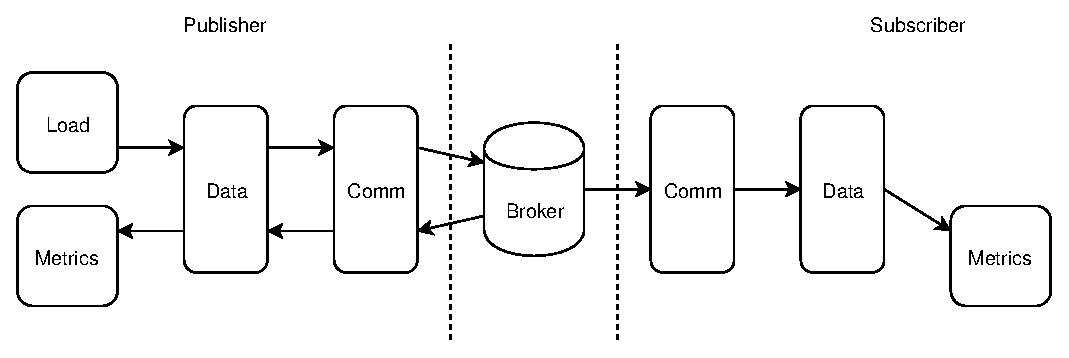
\includegraphics[width=\linewidth]{figures/benchmark_architecture.eps}
  \caption{Main architecture building blocks}
  \label{fig:benchmark_architecture}
\end{figure}

A user must be able to swap instances of a block as required. To achieve this, we defined interfaces (inputs and outputs) for all blocks. 

The \textit{load block} will enable different types of IoT scenarios to be programmed and dynamically changed, so that we can attempt to mimic varied real world scenarios. Again, this should be totally independent from any other block so that the same workloads can be used throughout all middlewares and protocols, providing a basis for comparison and ensuring high flexibility. 
    
The \textit{data block} is where the middleware specific functions reside, and each of these is responsible for implementing its data structure and bridging the gap to the protocols. When a new middleware is to be tested, one can leverage the existing functions, thereby speeding up the implementation process. A new middleware will be added as a new instance of the \textit{data block} so as to not interfere with the previous middlewares.

%Similarly to the \textit{data block}, the \textit{comm block} is designed so that the protocols (HTTP, CoAP, MQTT, etc) are independent, so that the same communication methods can be re-used. 
Next, we have the \textit{communication block} where the protocols, such as HTTP, CoAP, MQTT, are lodged. Each has its methods implemented, e.g. POST or GET, so that they are middleware independent and can be reused. If a new protocol is required, its methods can be implemented without interfering with the remaining structure.

During the test cycle, a set of defined values, such as times and publish request sizes, will be stored and fed into the \textit{metrics block}, which will extract metrics such as average publish time or generated traffic. New metrics can be added without affecting those that are already implemented, also keeping result compatibility. 

\subsection{OM2M Implementation}
In an initial step, we created an application to benchmark the OM2M middleware by abstracting our previous work~\cite{pereira_benchmarking_2018,cardoso_benchmarking_2017}, while keeping it as generic as possible to enable future middleware additions, following our architecture guidelines. This resulted in the structure visible in Fig.~\ref{fig:class_diagram_om2m}.

\begin{figure}[tbp!]
  \centering
  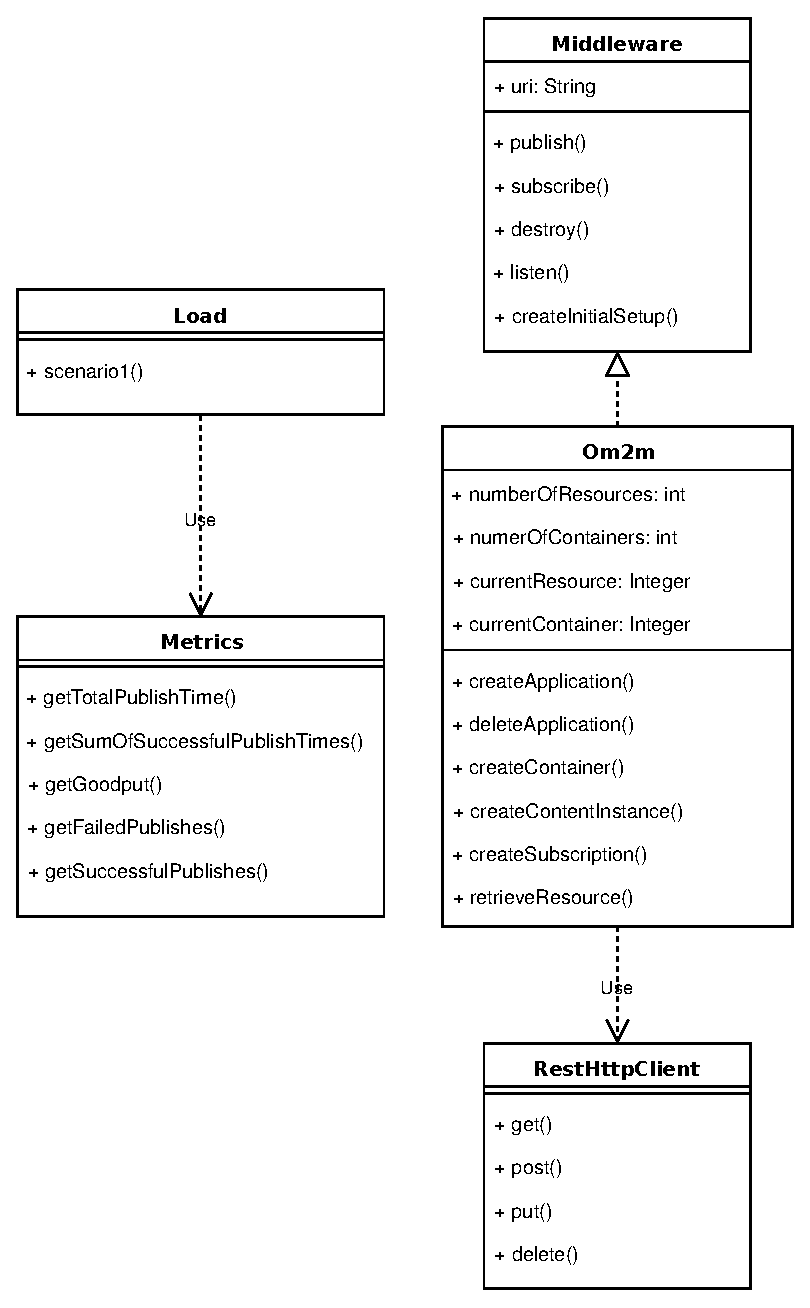
\includegraphics[width=\linewidth]{figures/class_diagram.eps}
  \caption{Class diagram for the initial platform stage}
  \label{fig:class_diagram_om2m}
\end{figure}

Since the load class will be performing the actual requests, it will also call upon the metrics class to get the results from the measurements. The load will consist of a certain number of publishes, with a certain message, at a given rate. All can be easily defined by the user. It is implemented by way of a loop, with each cycle corresponding to a publish request, with sleeps in between to meet the desired rate.

\begin{figure}[tbp!]
  \centering
  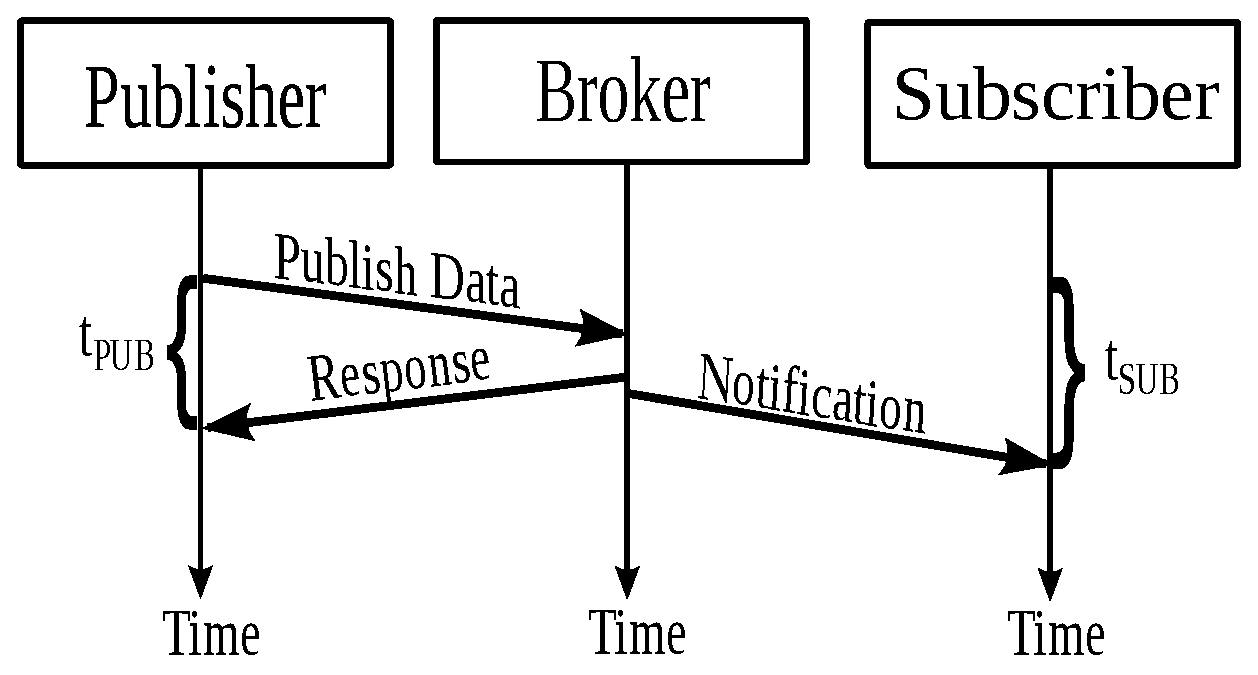
\includegraphics[width=\linewidth]{figures/pub_sub_time.eps}
  \caption{Publish and subscribe times~\cite{cardoso_benchmarking_2017}}
  \label{fig:pub_sub_time}
\end{figure}

The metrics currently implemented are \textit{publish and subscribe time}, both visible in Fig.~\ref{fig:pub_sub_time}, \textit{generated traffic}, \textit{failed and successful publishes}, \textit{size of a publish structure} and \textit{size of the URL}. Each \textit{publish time} is simply the difference between sending the request and receiving the response from the broker, easily implemented in the load class by measuring the elapsed time of a single cycle in the load loop.
\textit{Generated traffic} is measured by dividing the publish structure of each message by each publish time. The publish structure corresponds to the full message that is assembled by each middleware. Let's take the Om2m class as an example. Here, a publish request corresponds to the creation of a content instance of the container where we wish to publish. Therefore, the \textbf{createContentInstance()} method will take the message as input and create the appropriate data structure, such as in Listing~\ref{lst:application_creation} to create a content instance, to be sent as payload for a certain protocol, e.g., HTTP\@.

\begin{lstlisting}[linewidth=\columnwidth, caption=JSON payload for content instance creation, captionpos=b, label=lst:application_creation, language=json]
{
	"m2m:cin": {
		"con": "my_message-00000000000",
		"cnf": "application/json",
		"rn": "time_1520895952979"
	}
}
\end{lstlisting}
This will be returned to the calling publish method, in order for it to know the payload size for that particular middleware publish request. Since this class extends the \textbf{middleware} superclass, this method is always present and always has the same return values, providing generic metrics.
Following this, we have the \textit{failed and successful publishes}. In order to determine whether a certain request was successful or not, the response provided by the broker must be analysed. Naturally, this is protocol dependent, so in order to create a layer of abstraction, the basic communication methods of the used protocol, such as \textbf{POST} or \textbf{PUT} must return the broker response, in order for the Om2m class to be able to interpret if a publish was successful or not. This way, it will return to the main class a generic success or failure indicator, independent of protocol. 
Then, we have \textit{subscribe time} which is implemented differently, as it potentially relies on times registered at different machines. The subscriber must create a listener for the protocol it is expecting to receive in order to register the times. This listener will be in charge of registering the times at which the notifications arrive, meaning this metric is implemented at the protocol level. Lastly, we have the \textit{sizes of the publish structures and URL\@}. This metric aims to enable a user to see how much data needs to be added to the message that they want to send, as it can be significantly larger than the message itself, imposing a large overhead.

The goal of the \textbf{Middleware} superclass is to provide the methods that all middlewares are expected to implement and any attributes that are common as well. We therefore chose to have an \textbf{URI} to identify where it will be located on the network. The \textbf{publish()} and \textbf{subscribe()} methods are evident as we are dealing with publish/subscribe scenarios. The \textbf{createInitialSetup()} method is for registering resources, such as applications in the case of OM2M, the number of which is defined by the user. Next, we have \textbf{listen()}, which enables the subscriber to receive and parse notifications as needed, and register their arrival times. Finally, the \textbf{destroy()} method provides a way to clear any created resources so that the experiment may be conducted again on a clean broker. 

Finally, we come to the protocol classes. Currently, only HTTP is implemented in the \textbf{RestHttpClient()}, but others may be added in the future, such as CoAP or MQTT\@. The four methods in the \textbf{RestHttpClient} class are ubiquitous across several applications, and typically most middelwares which rely on HTTP will make use of these. 

\section{Evaluation}

\subsection{Adding new middlewares}

The platform development was conducted keeping in mind the extensibility to new middlewares. 
However, during such an extension, needs which were not accounted for can show up, and the platform must evolve to be able to accommodate them. In this section, we will see the changes to the architecture, and the differences and similarities between the implementation of OM2M and two additional middlewares: Fiware and Ponte. We will also highlight how much was reusable in terms of code and overall structure, and attempt to quantify the changes through the number of lines of code. 

\subsubsection{Fiware}

We decided to add the Fiware middleware as a result of previous work and greater familiarity with it. The class diagram is similar to that in Fig.~\ref{fig:class_diagram_om2m}. Since it is an extension of the \textbf{Middleware} superclass, it shares the five methods and attributes with \textbf{Om2m}; the rest is specific to this class, with a similar structure. The superclass methods will call the specific functions to bridge the gap to the communication protocol, in this case HTTP\@.
% Starting with \textbf{publish()}, the structure is identical, with only 4 lines out of 22 of code being different between both middlewares, which merely correspond to differing function calls and variable names. An Om2m publish calls the \textbf{createContentInstance()} function to create a new instance in a previously created container in an application, receiving the intended message and constructing a JSON payload in accordance to its standards, and sending it via an HTTP POST\@. Similarly, Fiware uses the \textbf{updateEntity()} method to update the current status of an entity, also constructing an appropriate JSON, but sending it with an HTTP PATCH. A key detail to note here is that using this method Fiware does not retain memory of previous status, as it is overwritten. Both of these methods return the JSON payloads and the HTTP response, and register the times at which the publishes were sent. The \textbf{subscribe()} method in both implementations is similar to this, but Fiware uses HTTP POST instead of a PATCH request.
% 
% The \textbf{listen()} function is the same in both, and creates an HTTP server for the subscriber to listen and parse the notifications.
% 
% Next, \textbf{destroy()} deletes all created resources so that it is easy to start from scratch. For this, Om2m calls \textbf{deleteApplication()} which takes the name of the resource to be deleted, constructs the JSON payload and POSTs it to the broker. For Fiware its \textbf{deleteEntity()}, and it works pretty much in the same way, the only change being the JSON created.
% 
% Finally we have \textbf{createInitialSetup()}, where resources are registered for the first time. For Om2m, a nested \textbf{for} loop is used to create the desired number of applications with \textbf{createApplication()}, and for each of these the number of containers with \textbf{createContainer()}. For FIWARE, the number of attributes must be defined upon entity creation, so these are handled at a lower level, at the \textbf{createEntity()} method, so only a simple \textbf{for} loop is used to create the necessary entities.
% 
Almost all functions used share the same structure: create the JSON to encapsulate the message, create the appropriate HTTP headers and make the HTTP request to the broker. This greatly eases the process of adding middlewares.

The default Fiware publish is an entity update. Fiware creates entities with certain attributes and updates them with each publish. Previous states are overwritten, thus it does not keep history. But which changes would be needed if we wanted to use Fiware with history? This would come down to what the user interprets as a publish request, but we could consider an entity creation as a publication itself. In this case, we would have to change the publish method to create an entity, instead of updating an existing one.

%Since entities remain in memory after their creation, if we consider the creation of an entity as a request, then the only necessary change would be to use \textbf{createEntity()} in the publish method, instead of \textbf{updateEntity()}. This would also render \textbf{createInitialSetup()} unnecessary, as entities would not have to be created beforehand. 
%
\subsubsection{Ponte}

Ponte is another implementation of the middleware superclass, so it shares the same methods as Fiware and OM2M.
As before, there is an URI identifier and two variables that indicate how many resources and attributes per resource this middleware instance will take. With Ponte, only the \textbf{publish()} and \textbf{createInitialSetup()} methods from the \textbf{Middleware} superclass were implemented. The reason for this is that there was no need to create an additional abstraction layer between the the middleware specific methods and the publish method as with other implementations. A plain HTTP PUT is required with the target resource and attribute in the URL, and the value as payload, without any need for JSON or XML marshalling.

\textbf{subscribe()} and \textbf{listen()} were not implemented as there is no way for the broker to notify a subscriber through HTTP\. The subscriber uses GET polling to check for notification. Thus, Ponte does not fully follow a publish/subscribe communication model.

There is no obvious way of deleting a resource, so \textbf{destroy} was also not implemented. The most obvious way to clean the deployment is a broker restart. 

\subsection{Impact on Code}

In order to better show the similarities between implementations, let's look at the publish methods themselves. In Fig.~\ref{fig:fiware_ponte_diff} we can see a comparison between both implementations for each middleware. The highlighted lines correspond to the differences.

\begin{figure}[tbp!]
  \centering
  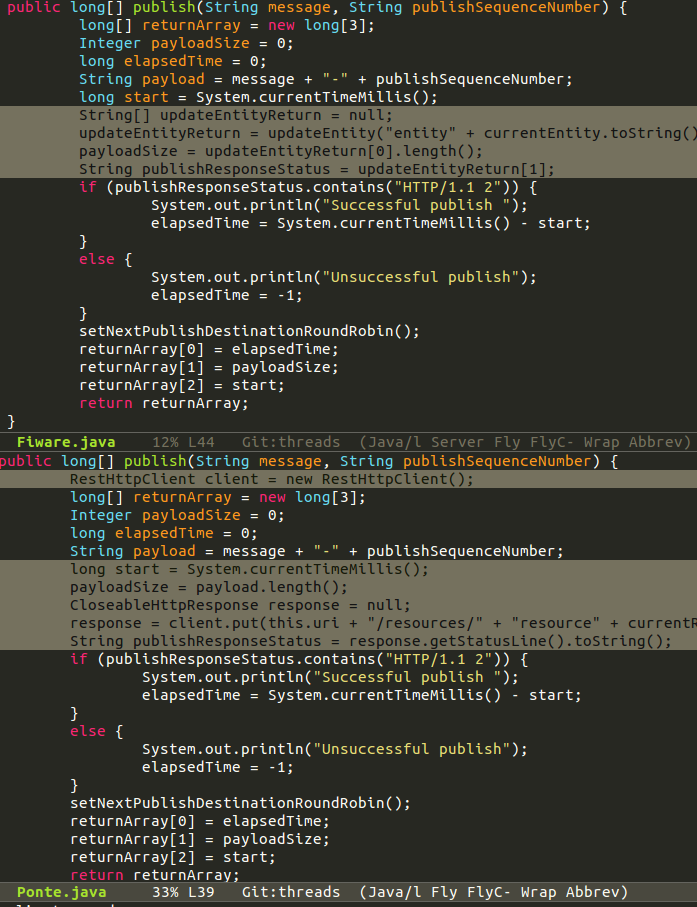
\includegraphics[width=\columnwidth]{figures/fiware_ponte_diff.png}
  \caption{Difference between Fiware (top) and Ponte (bottom) publish method}
  \label{fig:fiware_ponte_diff}
\end{figure}

The structure is identical, with the exception that Fiware calls an additional auxiliary method, \textbf{updateEntity()}, that assembles the JSON for the HTTP request that will execute the publish. Since Ponte does not need to assemble a payload in such a way, \textbf{put()} is called directly. This enabled an easy implementation for Ponte by analyzing what had been previously done for Fiware, speeding up the process of adding a new middleware.

\begin{table}[tbp!]
  \centering
  \caption{Lines of code for each class}
  \begin{tabular}{|c|c|}
    \hline 
    \textbf{Class} & \textbf{Lines of code} \\
    \hline 
    Main & 51 \\ 
    \hline
    Load & 119 \\
    \hline
    Middleware & 16 \\
    \hline
    Metrics & 136 \\
    \hline
    Ponte & 88 \\
    \hline
    Fiware & 193 \\
    \hline
    OM2M & 198 \\
    \hline
  \end{tabular}
  \vspace{1mm}
  \label{tab:lines_code}
\end{table}

We can attempt to quantify the changes needed for a new implementation by looking at the lines of code. The distribution of lines per class can be seen in Table~\ref{tab:lines_code}. 
This adds up to a total of 801. At first glance, we can see that for the implementation of a single middleware the effort required varies, with Ponte only needing 88 lines of new code. Nevertheless, there is a great deal that can be reused across all of them, greatly easing the process.% As we have seen previously, not only are the structures similar, but some of the methods are similar as well, such as with the \textbf{publish()} methods between Ponte and Fiware.

\section{Benchmarking Platform Validation}

The goal here is not to evaluate the performance of the platform, or to make a comparison with other middlewares. Rather, we use these results to validate the platform itself, show what type of information we can extract from these tests, while still keeping the platform generic.

The test consisted of 20000 publishes of 22 byte messages, at a maximum rate of 100 publishes per second. The subscriber and the broker were located on the same machine, while the publisher was separate. They were connected through 100 Mb/s Ethernet connections. In Fig.~\ref{fig:publish_times} we can see a comparison between the publish times of all three implemented middlewares. In Fig.~\ref{fig:subscribe_times} only Fiware and OM2M are present, as the subscribe times with Ponte using HTTP polling depend on the configuration of the polling interval. 
The other metrics are available in table~\ref{tab:misc_metrics_all_22} for each of them: the generated TCP traffic, total publish time, number of failed and successful publishes, size of a publish structure, and size of the URL.

\begin{figure}[tbp!]
  \centering
  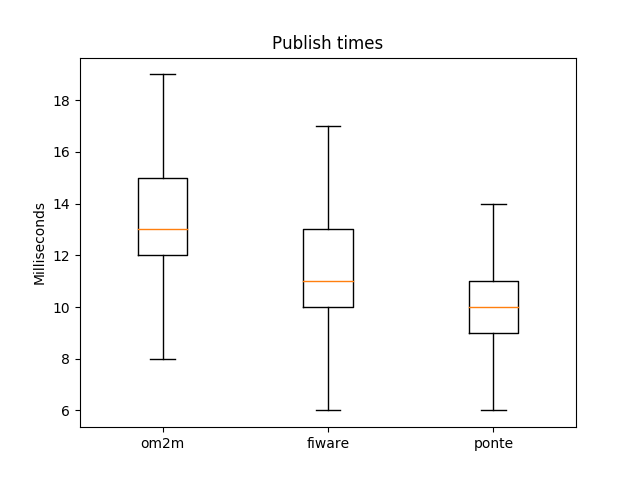
\includegraphics[width=\columnwidth]{figures/om2m_fiware_ponte_publish_times.png}
  \caption{Publish times for all three middlewares with 22 byte messages}
  \label{fig:publish_times}
\end{figure}

\begin{figure}[tbp!]
  \centering
  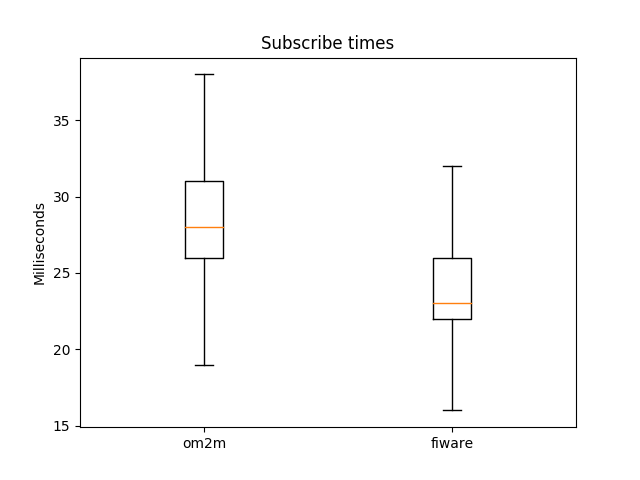
\includegraphics[width=\columnwidth]{figures/om2m_fiware_subscribe_times.png}
  \caption{Subscribe times for OM2M and Fiware with 22 byte messages}
  \label{fig:subscribe_times}
\end{figure}

\begin{table}[tbp!]
  \centering
  \caption{Results with 22 byte messages}
  \begin{tabular}{|c|c|c|c|}
    \hline 
    \textbf{Metrics} & \textbf{Fiware} & \textbf{OM2M} & \textbf{Ponte} \\
    \hline 
    Generated Traffic (KB/s) & 5.42 & 6.75 & 2.12 \\
    \hline 
    Failed publishes & 0 & 0 & 0 \\
    \hline 
    Successful publishes & 20000 & 20000 & 20000 \\
    \hline 
    Total publish time (s) & 259 & 283 & 208 \\
    \hline 
    Size of a publish structure & 70 & 95 & 22 \\
    \hline 
    Size of the URL (bytes) & 51 & 58 & 56 \\
    \hline 
    
  \end{tabular}
  \vspace{1mm}
  \label{tab:misc_metrics_all_22}
\end{table}

Changing parameters is merely altering the value of a few variables, depending on what the user wants. A second test was performed, using the same conditions as before, but with 10012 byte messages. The application can easily handle even large messages sizes such as in Fig.~\ref{fig:publish_times_10000}. The additional metrics can be seen in table~\ref{tab:misc_metrics_all_10012}. The platform would enable identifying with limited effort that OneM2M as configured would be less suited than the other two for periodic publications of a dataset with period less than 1 hour.

\begin{figure}[tbp!]
  \centering
  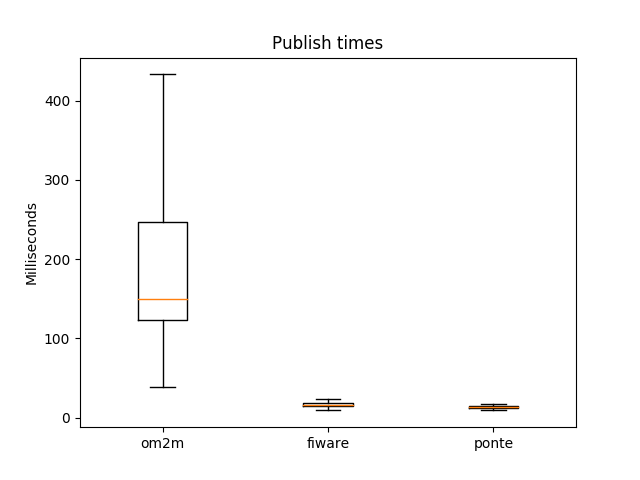
\includegraphics[width=\columnwidth]{figures/om2m_fiware_ponte_publish_times_10000.png}
  \caption{Publish times for all three middlewares with 10012 byte messages}
  \label{fig:publish_times_10000}
\end{figure}

\begin{figure}[tbp!]
  \centering
  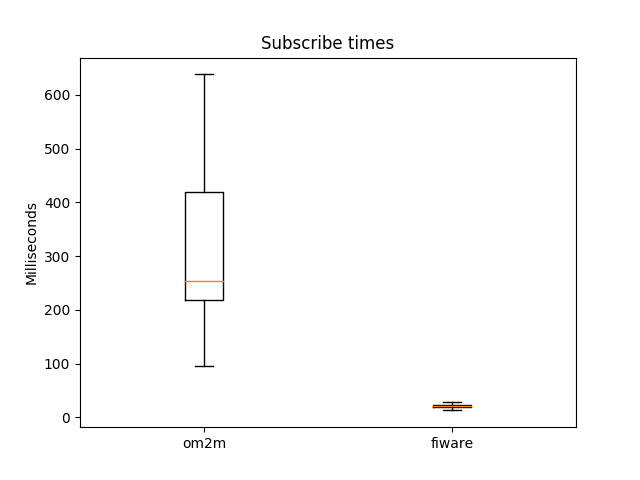
\includegraphics[width=\columnwidth]{figures/om2m_fiware_subscribe_times_10000.png}
  \caption{Subscribe times for OM2M and Fiware with 10012 byte messages}
  \label{fig:subscribe_times_10000}
\end{figure}


\begin{table}[tbp!]
  \centering
  \caption{Results with 10012 byte messages}
  \begin{tabular}{|c|c|c|c|}
    \hline 
    \textbf{Metrics} & \textbf{Fiware} & \textbf{OM2M} & \textbf{Ponte} \\
    \hline 
    Generated Traffic (KB/s) & 533.21 & 56.27 & 756.53 \\
    \hline 
    Failed publishes & 0 & 0 & 0 \\
    \hline 
    Successful publishes & 20000 & 20000 & 20000 \\
    \hline 
    Total publish time (s) & 380 & 3587 & 267 \\
    \hline 
    Size of a publish structure & 10060 & 10085 & 10012 \\
    \hline 
    Size of the URL (bytes) & 51 & 58 & 56 \\
    \hline 
    
  \end{tabular}
  \vspace{1mm}
  \label{tab:misc_metrics_all_10012}
\end{table}

We can observe that all middlewares use similar amount of Bytes for the resource, but we can see significant differences in the generated traffic, especially for large payloads. A large disparity in the total publish time could also be identified for the OM2M broker with large payloads. This is the type of issue that our benchmarking platform should enable to identify. 

\section{Limitations and Future Work}
For the time being the platform is implemented so as to allow extensions to new middleware to be straighforward and low effort, but there are areas where we can modularize the structure further. Taking again the example of Fig.~\ref{fig:fiware_ponte_diff}, we can see there are three distinct areas for a publish request: the assembly of the structure that will be sent, sending it using a certain communication protocol, and registering any relevant information from the response to implement metrics. Our goal is to create a further abstraction, so that only the structure assembly is required. 

Also, the platform is currently restricted to run in single threaded mode, but we intend to add multi-threaded support to enable simultaneous publishes. Also, additional metrics may need to be added, some of them protocol specific, to better compare different middlewares with the same communication protocol. 

\section{Conclusion}

In this paper, we proposed a scalable architecture for middleware benchmarking that targets pub/sub communication scenarios. We identified the common aspects between different middlewares, and factorized them, so as to avoid repeating the same steps across different experiments. We then created a platform based on this architecture and on previous experiments conducted with OM2M. After making sure it provided reliable metrics and results, we proceeded to add a new middleware, Fiware, and document the changes necessary for its implementation, both on an architecture level and on a platform level. We concluded that the architecture was adequate, and only one new class with 193 lines of code was necessary. We continued this process with the addition of Ponte, and the integration proved once more to be similar to the previous two, requiring only 88 new lines of code. On both occasions, the process was significantly quicker than it would have been if we were to create a specific application from scratch just for a single middleware. To prove the validity of our platform, we conducted two tests with different variables and obtained results with ease and, more importantly, assuring the same conditions across experiments, due to the nature of the application itself. This will allow for future users and researchers to have common ground in different tests, enhancing comparibility.

Future work should focus on better modularization for an easier implementation, multi-threaded support, and lower-level metrics at the TCP level. 

% trigger a \newpage just before the given reference
% number - used to balance the columns on the last page
% adjust value as needed - may need to be readjusted if
% the document is modified later
%\IEEEtriggeratref{8}
% The "triggered" command can be changed if desired:
%\IEEEtriggercmd{\enlargethispage{-5in}}

% references section

% can use a bibliography generated by BibTeX as a .bbl file
% BibTeX documentation can be easily obtained at:
% http://mirror.ctan.org/biblio/bibtex/contrib/doc/
% The IEEEtran BibTeX style support page is at:
% http://www.michaelshell.org/tex/ieeetran/bibtex/
%\bibliographystyle{IEEEtran}
% argument is your BibTeX string definitions and bibliography database(s)
%\bibliography{IEEEabrv,../bib/paper}
%
% <OR> manually copy in the resultant .bbl file
% set second argument of \begin to the number of references
% (used to reserve space for the reference number labels box)

\bibliographystyle{unsrt}
\bibliography{biblio}


% that's all folks
\end{document}


%%% Local Variables:
%%% mode: latex
%%% TeX-master: t
%%% End:


 